%% Author: Daniel Kaplan
%% Subject: Distributions (comparing different displays)




\providecommand{\HCode}[1]{#1} % dummy, just in case it's PDFlatex
\HCode{<link rel="stylesheet" href="fixSweave.css" type="text/css"
  media="screen" />}
\HCode{<link rel="stylesheet" href="http://dl.dropbox.com/u/5098197/Math135/RGuide/fixSweave.css" type="text/css"
 media="screen" />}


The plot shows two different displays of density.  The displays might
be from the same distribution or two different distributions.


\centerline{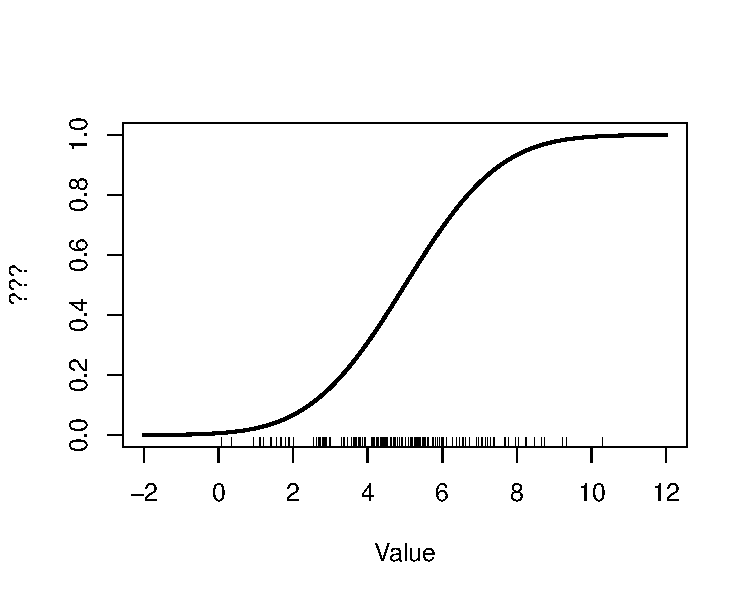
\includegraphics[width=4in]{Figures/B103-2-exp.pdf}}

\begin{enumerate}[(a)]
\item What are the two displays?

\begin{MultipleChoice}
\wrong{Density and cumulative}
\correct{Rug and cumulative}
\wrong{Cumulative and box plot}
\wrong{Density and rug plot}
\wrong{Rug and box plot}
\end{MultipleChoice}

\begin{AnswerText}
The rug plot is the small ticks on the horizontal axis.  The other
distribution has a shape that increases steadily --- never decreasing --- starting from 0 on
the left and going to 1 on the right.  That's the shape of a
cumulative distribution.  
\end{AnswerText}

\item 
The two displays show the same distribution. \TorF{true} 


\item Describe briefly any sign of mismatch or what features convince you
that the two displays are equivalent. \\
\TextEntry
\end{enumerate}

